\chapter{Pendahuluan}


\section{Latar Belakang}



Pasar modal Indonesia telah mengalami transformasi signifikan selama beberapa dekade terkahir ini. Pasar yang mulanya berskala kecil dengan jumlah emiten yang terbatas \parencite{OJK2007} kini berkembang menjadi gelanggang investasi yang lebih besar, lebih terdiversifikasi, dan lebih dikenal dalam kancah internasional\parencite{OECD2019}. Pembentukan Bursa Efek Indonesia (BEI) pada tahun 2007, yang merupakan penggabungan Bursa Efek Jakarta dan Bursa Efek Semarang, dan reformasi regulasi yang dilakukan oleh Otoritas Jasa Keuangan (OJK) menjadi salah satu batu loncatan dalam perkembangan pasar modal Indonesia.  Kepercayaan investor, baik lokal maupun asing, semakin kuat \parencite{Yuliani2017}, dan jumlah perusahaan dari berbagai sektor yang menawarkan sahamnya kian meningkat.
, dan jumlah perusahaan dari berbagai sektor yang menawarkan sahamnya kian meningkat.




    \begin{figure}[H]
        \centering
        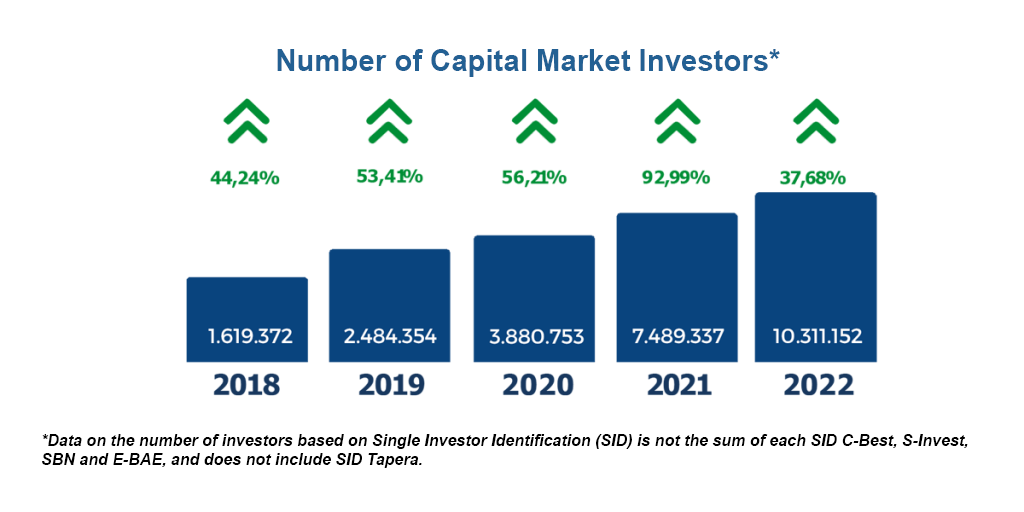
\includegraphics[width=0.8\textwidth]{resources/chapter-1-1.1-capitalmarketinvestor.png}
        \caption{Peningkatan Jumlah Investor di Indonesia \parencite{asiavesta2022}}  
    \end{figure}


    \begin{figure}[H]
        \centering
        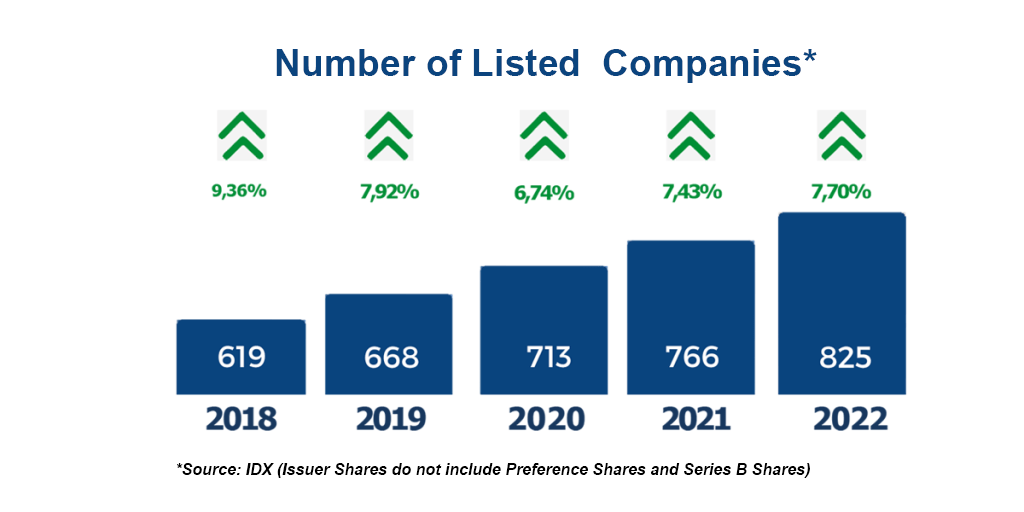
\includegraphics[width=0.8\textwidth]{resources/chapter-1-1.1-numberofcompanies.png}
        \caption{Peningkatan Jumlah Perusahaan di Pasar Modal \parencite{asiavesta2022}}
        \label{fig:number-of-companies}
    \end{figure}

Pertumbuhan ekonomi yang pesat dan upaya pembangunan infrastruktur yang masif turut menjadikan Indonesia target menarik bagi investor yang mencari peluang di pasar negara berkembang \parencite{WorldBank2023}. Bertumbuhnya ekonomi didampingi dengan masifnya upaya pembangunan infrastruktur di Indonesia menjadi faktor dalam menciptakan ekosistem bisnis yang positif. Akan tetapi, dinamika pasar Indonesia juga kompleks. Harga saham dipengaruhi oleh berbagai faktor seperti kebijakan pemerintah , indikator makroekonomi \parencite{IMF2022}, sentimen publik \parencite{FekrazadEtAl2022} , harga komoditas global \parencite{FAO2020}, serta perubahaan kondisi politik baik itu domestik ataupun mancanegara \parencite{BloomEtAl2019}. Hal ini membuat prediksi harga saham secara akurat menjadi rumit dikarenakan banyaknya variabel yang harus dikonsiderasi yang juga bersifat dinamik. 


Model statistik tradisional seperti ARIMA, VAR, ataupun GARCH telah lama digunakan untuk melakukan prediksi harga saham \parencite{NapitupuluWijaya2013}. Namun, model-model konvensional ini cenderung melihat hubungan antarvariabel secara linear dan tidak dapat mengakomodasi pola yang rumit dan dinamis \parencite{Goodfellow-et-al-2016}. Data keuangan biasanya tidak hanya dipengaruhi oleh satu ataupun dua vaktor, melainkan berbagai variabel, yang mungkin saling independen atau co-independen, yang tidak memiliki karakteritik linearitas antar keduanya tersebut \parencite{bhardwaj2022}. Hal ini membuat dibutuhkannya sebuah pendekatan yang dapat lebih fleksibel ataupun adaptif terhadap dinamika-dinamika data keuangan tersebut.

Dalam beberapa tahun terakhir, metode - metode yang digunakan untuk melakukan pelatihan pada model \textit{Machine Learning} dan \textit{Deep Learning} menjadi salah satu metode yang digunakan dalam melakukan pemodelan keuangan. Kekuatan utama dari teknik \textit{Deep Learning} adalah kemampuan model dalam mencari serta mempelajari pola - pola implisit yang terdapat di dalam data yang besar dan kompleks . \textit{Recurrent Neural Network} menjadi salah satu pilihan awal untuk melakukan pemodelan dalam \textit{Time series data}. Namun, arsitektur yang digunakan dalam \textit{RNN} biasanya memiliki masalah yaitu \textit{Vanishing Gradient} \parencite{Hochreiter1997} yang dapat membatasi kemampuan model dalam mencari pola dalam rentang waktu yang panjang.


Arsitektur \textit{Long Short-Term Memory} (LSTM) muncul sebagai solusi yang dapat mempertahankan informasi lokal dalam skala data yang panjang dengan mekanisme \textit{Gating} \parencite{Hochreiter1997}. Arsitektur \textit{Transformer} yang populer melalui \textit{paper} yang berjudul "Attention Is All You Need." membuka cara baru dalam melakukan \textit{modelling} pada data sekuensial \parencite{Vaswani2017}. Alih - alih melakukan \textit{data processing} secara berurutan seperti yang dilakukan oleh RNN, \textit{Transformer} menggunakan mekanisme \textit{attention} untuk menilai seberapa penting bagian tertentu dari data secara tepat sekuensial mengikuti urutan kronologis yang kaku. 

Seiring berkembangnya arsitektur \textit{Transformer}, muncul pula derivatif lainnya seperti  \textit{Temporal Fusion Transformer} (TFT) yang dirancang untuk dapat melakukan \textit{multi-horizon time series prediction}. TFT tidak hanya berfokus kepada tingkat dari akurasi prediksi, melainkan juga mempermudah interpretasi atau \textit{Model Understanding} \parencite{Lim2020}


Permasalahan utama dari prediksi pasar modal Indonesia adalah bagaimana cara memprediksi harga saham secara akurat dengan mengkonsiderasi banyak variabel yang saling independen ataupun co-independen serta perubahan dinamika pasar. Berbagai solusi telah dicoba seperti menggunakan model \textit{traditional statistical inference} sampai menggunakan model berbasiskan \textit{Deep Learning}. Pendekatan-pendekatan lainnya seperti ARIMA ataupun GARCH dapat juga menawarkan kemudahan serta interpretabilitas dari model yang sederhana namun tidak dapat menangani untuk mencari pola nonlinear. Sementara itu, model \textit{Deep Learning} seperti LSTM dapat memberikan peningkatan performa dalam menangkap pola intrinsik yang mungkin terdapat pada data \textit{Time series}.

Penelitian ini berfokus pada pembandingan implementasi model dengan arsitektur \textit{Temporal Fusion Transformer} dengan implementasi model dengan arsitektur \textit{Long Short-Term Memory} dengan varian - varian modernnya. 


\section{Rumusan Masalah}

Berdasarkan latar belakang yang sudah dijelaskan sebelumnya, berikut adalah rumusan masalah yang diajukan.

\begin{enumerate}
    \item Bagaimana cara mengimplementasikan model dengan arsitektur \textit{Temporal Fusion Transfomer} pada data \textit{Time Series} pasar saham Indonesia ?
    \item Bagaimana cara mengimplementasikan model dengan varian-varian arsitektur \textit{Long Short-Term Memory} pada data \textit{Time Series} pasar saham Indonesia ?
    \item Bagaimana perbandingan performa kinerja antara model dengan arsitektur \textit{Temporal Fusion Transformer} dan \textit{Long Short-Term Memory} dengan varian-variannya?
    \item Fitur-fitur apa saja yang dapat membuat suatu model memiliki performa yang lebih baik serta apa hubungan antara fitur yang digunakan dengan performa model tersebut ?
\end{enumerate}

\section{Tujuan}

Berdasarkan rumusan masalah yang sudah dijelaskan sebelumnya, berikut adalah tujuan dari penelitian ini.

\begin{enumerate}
  \item Membuat model dengan arsitektur TFT dan varian LSTM pada data \textit{time series} pasar saham Indonesia.
 \item Mengevaluasi hasil performa dari model yang menggunakan arsitektur TFT dan varian LSTM pada data \textit{time series} pasar saham Indonesia.
  \item Menentukan fitur-fitur yang menjadi alasan mengapa salah satu model memiliki performa yang lebih baik daripada model lainnya pada data \textit{time series} pasar saham Indonesia.
\end{enumerate}

\section{Batasan Masalah}

Adapun beberapa batasan masalah yang diterapkan untuk penyusunan tugas akhir ini adalah sebagai berikut.
\begin{enumerate}
\item Dataset yang digunakan adalah data yang berasal dari\href{https://pypi.org/project/yfinance}{ Yahoo! Finance API } dan juga data-data perusahaan yang terdaftar pada Bursa Efek Indonesia \href{https://www.idx.co.id/en/market-data/stocks-data/stock-list}{https://www.idx.co.id/en/market-data/stocks-data/stock-list} 
\item Bahasa pemrograman yang digunakan dalam melakukan pengembangan model dengan arsitektur TFT dan varian LSTM adalah Python 3.
\item Penelitian ini dilakukan menggunakan \textit{device} Laptop Lenovo Legion 5 15IMH05 serta layanan \textit{cloud computing} yaitu Google Colab. 
\end{enumerate}


\section{Metodologi}

Metodologi yang dipakai dalam penelitian kali ini adalah \textit{Cross-Industry Process for Data Mining} (CRISP-DM). CRISP-DM merupakan salah satu metodologi umum yang digunakan dalam pengembangan projek \textit{data science} dikarenakan fase-fasenya yang fleksible untuk dilakukan sehingga cocok untuk digeneralisir kepada setiap domain-domain bisnis yang membutuhkan \parencite{datasciencecentral2024}. Metodologi ini terdiri atas 6 fase sesuai dengan gambar \ref{fig:crispdm-method}.

    \begin{figure}[H]
        \centering
        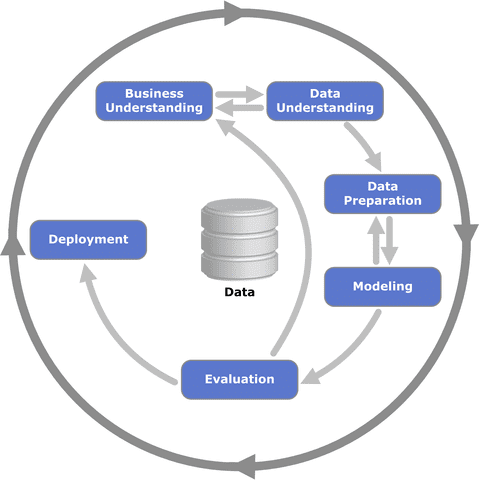
\includegraphics[width=0.8\textwidth]{resources/chapter-1-1.5-crispdm.png}
        \caption{Metodologi CRISP-DM. Sumber: \parencite{datasciencecentral2024}}
        \label{fig:crispdm-method}
    \end{figure}

\begin{enumerate}
\item \textbf{Business Understanding} \\
Fase pertama dalam CRISP-DM adalah memahami tujuan bisnis yang diinginkan dan mengidentifikasi masalah bisnis yang ingin diselesaikan. Tujuan utama tahap ini adalah agar selarasnya solusi projek \textit{data science} dengan masalah bisnis yang ingin diselesaikan. 
\item \textbf{Data Understanding} \\
Fase kedua adalam CRISP-DM adalah mengumpulkan data, memahami kualitas, struktur, serta relevansi, serta feasibilitas dari data yang akan digunakan untuk pemgembangan proyek. 
\item \textbf{Data Preparation} \\
Fase ketiga dalam CRISP-DM adalah melakukan pengolahan data untuk digunakan untuk fase selanjutnya.
\item \textbf{Modelling} \\
fase keempat dalam RISP-DM adalah membangun model \textit{machine learning} menggunakan algoritma yang sesuai dan data yang sudah dipersiapkan dari tahap sebelumnya. 
\item \textbf{Evaluation} \\
Fase kelima dalam CRISP-DM adalah melakukan evaluasi performa dari model yang telah dibuat dari fase sebelumnya. Apabila model yang telah dibuat memiliki performa yang kurang memuaskan, maka iterasi dapat diulang kembali ke salah satu fase sebelumnya. 
\item \textbf{Deployment} \\
Fase terakhir dalam CRISP-DM adalah melakukan \textit{deployment} dari model yang kita gunakan sehingga model yang sudah dibuat dapat diakses atau digunakan. 
\end{enumerate}
